% ============================================================
%  SPÉCIFICATION — specification.tex
% ============================================================
\section{Spécification du simulateur}
\label{sec:specification}

Cette section détaille les fonctionnalités attendues du projet ainsi que les
contraintes qui définissent son comportement. Elle constitue le référentiel
fonctionnel sur lequel s'appuie la conception décrite dans la
section~\ref{sec:realisation}.

% ------------------------------------------------------------
\subsection{Notions de base et contraintes du projet}
\label{subsec:notions_base}

Cette sous-section définit les fondements du modèle de simulation, établit le
vocabulaire technique utilisé dans l'ensemble du rapport et recense les
limitations connues de l'application.

\paragraph{Fonctionnement général du logiciel.}
Le fonctionnement repose sur un modèle de simulation par \emph{rounds} successifs.
À chaque round, le système exécute un cycle complet divisé en quatre étapes
distinctes, comme l'illustre la figure~\ref{fig:flux_round}.

\begin{figure}[H]
  \centering
  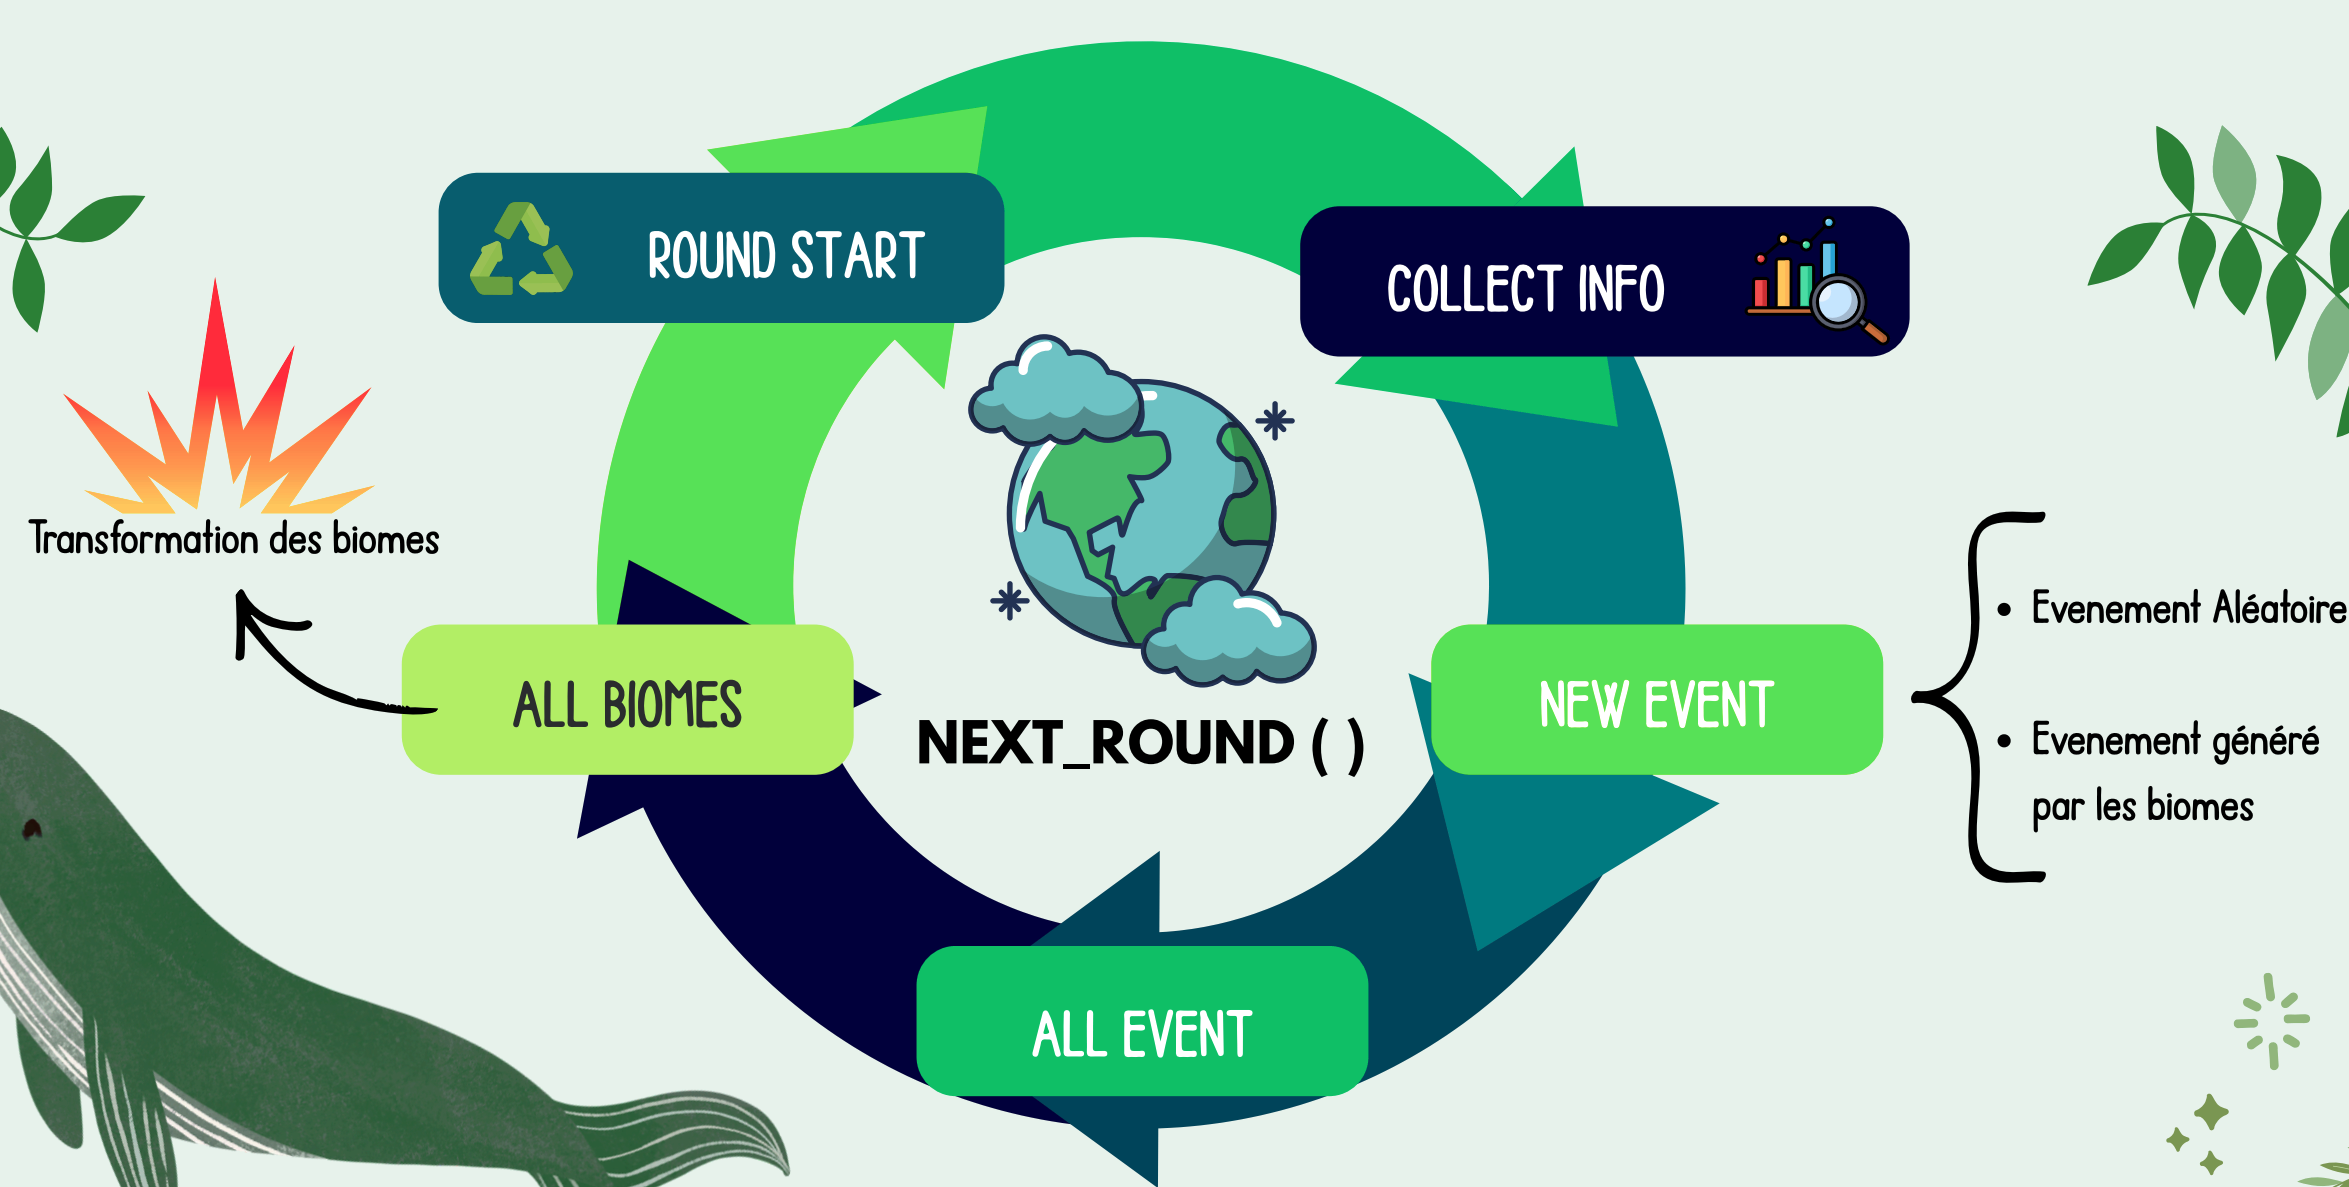
\includegraphics[width=0.75\textwidth]{images/flux_round.png}
  \caption{Flux d'exécution d'un round de simulation}
  \label{fig:flux_round}
\end{figure}

\begin{enumerate}
  \item \textbf{Génération d'événements}~: au début de chaque round, de nouveaux
    événements météorologiques apparaissent aléatoirement sur la carte selon des
    probabilités configurables.
  \item \textbf{Déplacement des événements}~: les événements mobiles se déplacent
    d'une case dans leur direction assignée~; ce déplacement peut être bloqué par
    les biomes Montagne.
  \item \textbf{Application des impacts}~: les événements modifient les propriétés
    numériques des biomes qu'ils occupent.
  \item \textbf{Évaluation des transformations}~: les règles de transformation
    vérifient les propriétés de chaque biome~; si les conditions sont satisfaites,
    le biome se transforme en un autre type.
\end{enumerate}

La carte est représentée par une grille bidimensionnelle configurable dont chaque
cellule contient exactement un biome. Chaque biome possède quatre propriétés
numériques bornées entre~0 et~100~: température, humidité, pollution et
purification.

\paragraph{Vocabulaire et terminologies de base.}
Les termes techniques récurrents dans ce rapport sont définis comme suit.

\begin{itemize}
  \item \textbf{Biome}~: unité de base de la carte représentant un type
    d'écosystème distinct (Forêt, Désert, Mer, Montagne, Banquise, Ville,
    Village).
  \item \textbf{Round}~: cycle d'exécution de la simulation comprenant les quatre
    étapes de génération, déplacement, impact et transformation.
  \item \textbf{Événement}~: phénomène météorologique affectant les propriétés
    numériques des biomes (Pluie, VentFroid, VentChaud, Pollution, etc.).
  \item \textbf{Transformation}~: changement automatique d'un biome vers un autre
    type selon les règles écologiques définies.
  \item \textbf{Carte}~: grille bidimensionnelle de blocs, chaque bloc contenant
    un biome identifié par ses coordonnées $(x, y)$.
  \item \textbf{Propriétés}~: les quatre caractéristiques numériques d'un biome,
    à savoir la température, l'humidité, la pollution et la purification.
\end{itemize}

\paragraph{Contraintes et limitations connues.}
L'application présente plusieurs contraintes et limitations identifiées lors de
son développement.

La première limitation concerne l'\textbf{absence de persistance des données}.
L'état de l'écosystème est intégralement géré en mémoire vive durant l'exécution.
Le logiciel ne dispose pas de mécanisme de sérialisation permettant de sauvegarder
l'état d'une simulation pour la reprendre ultérieurement.

La deuxième limitation porte sur les \textbf{contraintes de l'interface
Homme-Machine}. L'interface graphique possède une résolution fixée à
1920\,$\times$\,1080~pixels. Le positionnement absolu des composants Swing empêche
un redimensionnement dynamique de la fenêtre, et l'ergonomie du mode édition ne
prend pas en charge la sélection de masse ni la duplication de zones.

La troisième limitation concerne le \textbf{couplage entre le moteur et
l'interface graphique}. Le gestionnaire de simulation (\texttt{ManageurBasique})
communique directement avec certains composants Swing, ce qui crée une dépendance
bidirectionnelle entre la logique métier et la couche de présentation. Ce couplage
rend le remplacement ou le test isolé du moteur plus complexe qu'avec une
architecture entièrement découplée.

La quatrième limitation est l'\textbf{absence de parallélisme dans le moteur de
simulation}. Toutes les étapes d'un round~--- génération, déplacement, impact et
transformation~--- s'exécutent séquentiellement dans un unique thread. Sur des
cartes de grande taille ou avec un nombre d'entités élevé, cette approche
séquentielle constitue un goulot d'étranglement, car les interactions entre
événements et biomes ne tirent aucun parti du multi-cœur du processeur.

% ------------------------------------------------------------
\subsection{Fonctionnalités attendues du projet}
\label{subsec:fonctionnalites}

Cette sous-section recense l'ensemble des fonctionnalités que l'application doit
implémenter, organisées par domaine fonctionnel.

\paragraph{Gestion de la carte.}
La carte est représentée par une grille bidimensionnelle de cellules appelées
\emph{blocs}. Chaque bloc contient un biome et est identifié par ses coordonnées
$(x, y)$. Les dimensions de la grille sont configurables (par exemple
$20 \times 20$ ou $30 \times 30$). La figure~\ref{fig:grille_biome} montre un
exemple de grille peuplée de biomes variés.

\begin{figure}[H]
  \centering
  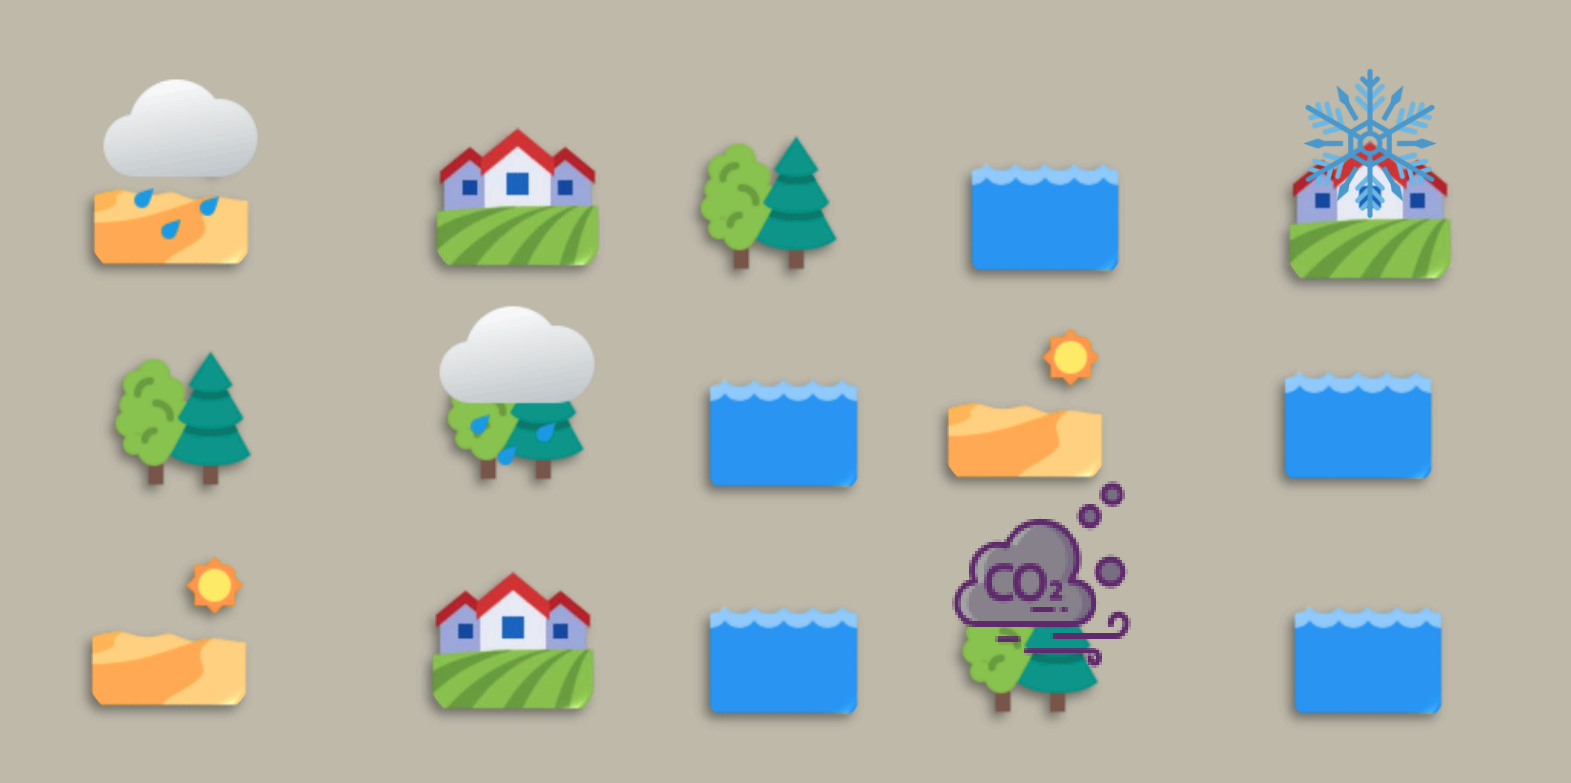
\includegraphics[width=0.7\textwidth]{images/grille_biome.png}
  \caption{Exemple de grille de biomes générée par l'application}
  \label{fig:grille_biome}
\end{figure}

La génération de la carte peut s'effectuer de manière aléatoire, les probabilités
de chaque type de biome étant définies dans le fichier de configuration. Chaque bloc
est accessible et modifiable via des méthodes d'accès dédiées. Les coordonnées sont
validées avant tout accès pour garantir la cohérence des données.

\paragraph{Gestion des biomes.}
L'application modélise sept types de biomes, chacun représentant un écosystème
distinct avec des propriétés environnementales spécifiques (température, humidité,
pollution, purification). La Montagne constitue une exception notable~: elle est
immuable et ne peut être transformée par aucune règle. Les transformations entre
biomes suivent des chaînes logiques reflétant des phénomènes écologiques
plausibles~; par exemple, une Forêt soumise à la désertification devient un Désert,
lequel peut, sous l'effet inverse de la forestation, redevenir une Forêt. Les
valeurs initiales des propriétés de chaque biome et leur hiérarchie d'implémentation
sont présentées dans la section~\ref{sec:realisation}.

\paragraph{Gestion des événements.}
L'application gère treize types d'événements divisés en deux catégories. Les
événements statiques restent à une position fixe pendant leur durée de vie~; le
Météore est le seul représentant de cette catégorie. Les événements mobiles se
déplacent d'une case à chaque round dans une direction assignée. Le
tableau~\ref{tab:evenements} synthétise les propriétés de chaque événement.

\begin{table}[H]
  \centering
  \caption{Propriétés des événements météorologiques}
  \label{tab:evenements}
  \begin{tabular}{llrrrr>{\small}r}
    \toprule
    \textbf{Événement} & \textbf{Catégorie} & \textbf{Durée}
      & $\Delta$\textbf{Temp.} & $\Delta$\textbf{Hum.}
      & $\Delta$\textbf{Poll.} & $\Delta$\textbf{Purif.} \\
    \midrule
    Pluie         & Mobile  &  4 &   0   & $+$5  &   0   &  0 \\
    VentFroid     & Mobile  &  4 & $-$5  &   0   &   0   &  0 \\
    Pollution     & Mobile  &  4 &   0   &   0   & $+$10 &  0 \\
    Purification  & Mobile  &  4 &   0   &   0   &   0   & $+$5 \\
    Météore       & Statique & 20 & $+$50 &   0   & $+$20 &  0 \\
    Orage         & Mobile  &  6 &   0   & $+$10 &   0   &  0 \\
    Grêle         & Mobile  &  3 & $-$10 & $+$5  &   0   &  0 \\
    Tornade       & Mobile  &  8 &   0   & $+$5  & $+$5  &  0 \\
    PluieBénite   & Mobile  &  5 &   0   & $+$8  & $-$5  & $+$10 \\
    Zéphyr        & Mobile  &  3 & $+$5  &   0   &   0   &  0 \\
    Tonnerre      & Mobile  &  2 &   0   & $+$8  &   0   &  0 \\
    Smog          & Mobile  &  6 &   0   &   0   & $+$15 &  0 \\
    NuageToxique  & Mobile  &  7 &   0   &   0   & $+$20 &  0 \\
    \bottomrule
  \end{tabular}
\end{table}

Comme le montre le tableau~\ref{tab:evenements}, les événements mobiles exercent
des impacts différenciés sur les quatre propriétés des biomes. Chaque événement
mobile possède une durée de vie~; à son expiration, il est retiré de la carte.
Lorsqu'un déplacement est bloqué par une Montagne, l'événement choisit une
nouvelle direction aléatoire~; s'il n'en existe aucune, il reste en place.

Chaque événement est généré selon une formation spatiale définie, lui conférant
une empreinte visuelle reconnaissable sur la grille. Le
tableau~\ref{tab:formations} détaille la formation associée à chaque type
d'événement.

\begin{table}[H]
  \centering
  \caption{Formations spatiales des événements météorologiques}
  \label{tab:formations}
  \begin{tabular}{ll}
    \toprule
    \textbf{Événement} & \textbf{Formation} \\
    \midrule
    Pluie, PluieAcide, Orage, PluieBénite & Carré 2$\times$2 \\
    VentFroid, VentChaud & Ligne horizontale \\
    Grêle & Ligne verticale \\
    Tornade & Croix \\
    Zéphyr & Diagonale \\
    Tonnerre & Forme en T \\
    Smog, NuageToxique & Cercle \\
    Pollution, Purification, Météore & Unique \\
    \bottomrule
  \end{tabular}
\end{table}

\paragraph{Système de transformation des biomes.}
Six règles de transformation écologique contrôlent l'évolution des biomes au fil
des rounds. Le tableau~\ref{tab:transformations} présente les conditions
d'activation de chaque règle et le biome cible associé.

\begin{table}[H]
  \centering
  \caption{Règles de transformation écologique et conditions d'activation}
  \label{tab:transformations}
  \begin{tabular}{llp{7cm}}
    \toprule
    \textbf{Règle} & \textbf{Biome cible} & \textbf{Condition principale} \\
    \midrule
    Inondation      & Mer      & Humidité $\geq 90$, Temp.\ $\geq 5$, Poll.\ $\leq 40$ \\
    Glaciation      & Banquise & Temp.\ $\leq 0$, Hum.\ $\geq 20$, Poll.\ $\leq 20$ \\
    Désertification & Désert   & Temp.\ $\geq 50$ ou Hum.\ $\leq 10$ \\
    Forestation     & Forêt    & Temp.\ $\in [10, 35]$, Hum.\ $\in [60, 90]$, Poll.\ $\leq 25$ \\
    Civilisation    & Village  & Temp.\ $\in [15, 40]$, Hum.\ $\in [20, 80]$, Poll.\ $\leq 10$ \\
    Densification   & Ville    & Temp.\ $\in [18, 45]$, Hum.\ $\in [30, 70]$, Poll.\ $\in [10, 60]$ \\
    \bottomrule
  \end{tabular}
\end{table}

Les conditions décrites dans le tableau~\ref{tab:transformations} sont évaluées à
chaque round pour chaque biome de la carte. Chaque règle est implémentée sous
forme d'un objet indépendant, ce qui garantit leur évaluation uniforme par le
moteur de simulation sans modification de l'algorithme principal.

\paragraph{Interface graphique.}
L'interface graphique permet de visualiser et de contrôler la simulation en temps
réel. La carte est affichée sous forme de grille colorée où chaque cellule
représente un biome distinct. Les événements sont superposés à la grille sous forme
de symboles animés. L'interface propose les contrôles suivants~: Play pour démarrer
la simulation, Pause pour la suspendre, Vitesse~$\times 2$ pour accélérer
l'exécution, Bilan de fin pour consulter le récapitulatif, et Statistiques pour
ouvrir la fenêtre d'analyse détaillée. Un mode édition permet de modifier
manuellement les biomes avant ou pendant la simulation. Une fenêtre de tutoriel
est également disponible pour guider l'utilisateur lors de sa première utilisation.
